
\documentclass[preprint,12pt]{elsarticle}

\usepackage[spanish]{babel}
\usepackage{amssymb}
\usepackage{graphicx}
\usepackage{lineno}
\usepackage[utf8]{inputenc}
\usepackage{url}
\usepackage{natbib} 
\usepackage{amsmath} 
\usepackage{amssymb} 

\begin{document}
	
	\begin{frontmatter} 

		\title{\huge MAPEO OBJETO RELACIONAL}
		
		\author{Estrella Palacios, Katherine Lizbeth              	(2016056193))}
		\author{Gonzales Cave, Angel Gabriel              	(2017057861))}
		\author{Huichi Contreras, Franklin Carlos         	(2016054948))} 
		\author{Huillca Umpiri, Willian Arturo             		(2015053793))} 
		\address{Escuela Profesional de Ingeniería de Sistemas}
		\address{Universidad Privada de Tacna}
		\address{Tacna, Perú}
		
%% ABSTRACT --------------------------------------------------------------------------------------------------------------------

		\begin{abstract}
		
Object Relational Mapping (also known as ORM or OR mapping) is a process that involves the transformation between object and relational models and between the systems that support these methodologies.
In order to carry out this transformation it is necessary to have a broad knowledge of object-oriented and relational technologies, as well as their similarities and differences.

		\end{abstract}

%% ----------------------------------------------------------------------------------------------------------------------------------

	\end{frontmatter}

%% RESUMEN ---------------------------------------------------------------------------------------------------------------------

\section{Resumen}

El mapeo objeto/relacional (también conocido como ORM o OR mapping) es un proceso que consiste en la transformación entre modelos de objetos y relacional y entre los sistemas que soportan estas metodologías.
Para poder realizar esta transformación es necesario tener un amplio conocimiento de las tecnologías orientada a objetos y relacional, así como también de sus similitudes y diferencias.

%% ----------------------------------------------------------------------------------------------------------------------------------


%% INTRODUCION ----------------------------------------------------------------------------------------------------------------

\section{Introducción} 
Varias áreas de aplicaciones para los sistemas de bases de datos se hallan limitadas por las restricciones del modelo de datos relacional. El modelo relacional orientado a objetos combina caracteristicas del modelo relacional y del modelo orientado a objetos. Este modelo proporciona un sistema de tipos de datos variado. Aplica la herencia a las relaciones, no sólo a los tipos.\\El modelo de datos relacional orientado a objetos permite una migración fácil desde las bases de datos relacionales.
El término base de datos orientada a objetos se utiliza para describir los sistemas de bases de datos que soportan el acceso directo a los datos desde lenguajes de programación orientados a objetos, sin necesidad de lenguajes de consultas relacionales como interfaz de las bases de datos.

%% ----------------------------------------------------------------------------------------------------------------------------------


%% MARCO TEÓRICO ------------------------------------------------------------------------------------------------------------

\section{Marco Teórico}

%% PRIMERA SUBSECCION 

\subsection {\textbf{Concepto del ORM}}

Bauer y King señalan que el mapeo Objeto/Relacional es “la persistencia automatizada y transparente de las tablas en una Base de Datos relacional, usando metadatos que definen el mapeo entre los objetos y la Base de Datos” \cite{BauerKing2005} 

Un ORM es un modelo de programación que permite mapear las estructuras de una base de datos relacional (SQL Server, Oracle, MySQL, etc.), en adelante RDBMS (Relational Database Management System), sobre una estructura lógica de entidades con el objeto de simplificar y acelerar el desarrollo de nuestras aplicaciones.\cite{Deloitte1} 

% Las estructuras de la base de datos relacional quedan vinculadas con las entidades lógicas o base de datos virtual definida en el ORM, de tal modo que las acciones CRUD (Create, Read, Update, Delete) a ejecutar sobre la base de datos física se realizan de forma indirecta por medio del ORM.

% La consecuencia más directa que se infiere del párrafo anterior es que, además de “mapear”, los ORMs tienden a “liberarnos” de la escritura o generación manual de código SQL (Structured Query Language) necesario para realizar las queries o consultas y gestionar la persistencia de datos en el RDBMS.

% Así, los objetos o entidades de la base de datos virtual creada en nuestro ORM podrán ser manipulados por medio de algún lenguaje de nuestro interés según el tipo de ORM utilizado, por ejemplo, LINQ sobre Entity Framework de Microsoft. La interacción con el RDBMS quedará delegada en los métodos de actualización correspondientes proporcionados por el ORM. Los ORMs más completos ofrecen servicios para persistir todos los cambios en los estados de las entidades, previo seguimiento o tracking automático, sin escribir una sola línea de SQL. 

\begin{figure}[htb]
	\begin{center}
		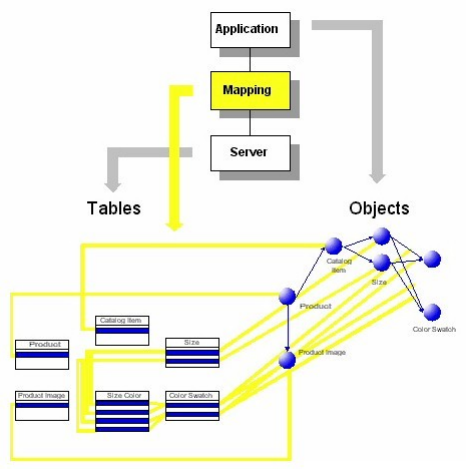
\includegraphics[width=7.5cm]{./IMAGENES/ORM} 
		\caption{Mapeo Objeto/Relacional}
	\end{center}
\end{figure}


\subsection {\textbf{Ventajas y Desventajas del ORM\\}}


\subsubsection{\textbf{Ventajas}}
Algunas de las ventajas del ORM son: \cite{Borja2010} \cite{Polo2013} 

\begin{itemize}

	\item Rapidez de desarrollo 
% ORM permite crear un modelo ajustado ya que leeautomáticamente el esquema de tablas y relaciones.
	\item Abstracción de la base de datos 
% Ayuda a que automáticamente las consultas que se realicen en la base de datos se conviertan de registros aobjetos y viceversa y de esta forma adaptarse a los proveedores: (MYSQL,ORACLE, POSTRESQL, ETC.).
	\item Lenguaje propio para consultas a la base de datos
% Las herramientas queofrece ORM para poder extraer los datos de la forma que se necesita (filtros,ordenaciones, agrupaciones.
	\item Encapsulación 
% Encapsula la lógica de los datos pudiendo hacer cambios queafectan a toda la aplicación únicamente modificando una función.
	\item Portabilidad 
% Permite cambiar en un proyecto el tipo de proveedor de unabase de datos MySQL a una Oracle sin ningún tipo de complicación.
	\item Reutilización
% Permite llamar a los métodos de un objeto de datos desdedistintas partes de la aplicación e incluso desde diferentes aplicaciones.
	\item Seguridad
% Permite proteger las aplicaciones de los ataques más comunescomo SQL Injections.
	\item Mantenimiento del código
% La correcta ordenación de la capa de datos permitemodificar y mantener el código

\end{itemize}

\subsubsection{\textbf{Desventajas}}

Algunas de las desventajas del ORM son: \cite{Borja2010} \cite{Polo2013} 

\begin{itemize}

	\item Tiempo utilizado en el aprendizaje
% Su curva de aprendizaje es amplia debido a la gran variedad de librerías queofrece ORM explorar la totalidad de su rendimiento costaría tiempo, sepuede usar en un proyecto de poca complejidad para un excelenterendimiento.
% Este tipo de herramientas suelen ser complejas por lo que su correcta utilización lleva un tiempo que hay que emplear en ver el funcionamiento correcto y ver todo el partido que se le puede sacar.
	\item Aplicaciones algo más lentas
% Esto es debido a que todas las consultas que se hagan sobre la base de datos, el sistema primero deberá de transformarlas al lenguaje propio de la herramienta, luego leer los registros y por último crear los objetos.

\end{itemize}

\subsection{\textbf{ORMs en el mercado actual\\}}

\begin{itemize}
	
	\item \textbf{Microsoft Entity Framework 6.0:} \\Microsoft Entity Framework se publicó por primera vez en 2008, como parte de .NET Framework 3.5 SP1 y Visual Studio 2008 SP1. A partir de la versión 4.1, se ha distribuido como paquete NuGet independiente convirtiéndose en uno de los más populares en NuGet.org. Sólo para plataforma Windows. Muy estable. Open Source. Proporciona servicios avanzados de modelado y seguimiento de estados de entidades, persistencia automática de cambios, caching, gestión de transacciones, etc.
	
	\item \textbf{Microsoft Entity Framework Core 2.0:} \\Nueva implementación de Entity Framework en versión Core. Más ligera, extensible y multiplataforma (Windows, Linux, Mac). Ofrece un rendimiento más potente en comparación con la versión desarrollada específicamente para .Net Framework. En continua evolución. Open Source. Puede ejecutarse sobre .Net Framework 4.6.1, .Net Core 2.0 o posteriores. 
	
	\item \textbf{Microsoft Entity Framework Core 2.1:} \\Versión más reciente de Entity Framework Core lanzada a finales de mayo de 2018. Incluye mejoras funcionales y de rendimiento, así como correcciones sobre la versión anterior. No obstante, no toda la funcionalidad de Entity Framework 6.0 ha sido migrada todavía a esta última versión de Entity Framework Core.
	
	\item \textbf{NHibernate:} \\Conversión de Hibernate en Java para lenguaje C\# compatible con plataforma .Net. Estable. Open Source.
		
	\item \textbf{Dapper:} \\Micro-ORM que proporciona métodos de extensión a las clases de .Net Framework para mapear resultados y persistir datos, previa inyección de código SQL personalizado. No nos libera pues de la implementación de nuestro código SQL, actuando como simple mapeador, pero a cambio ofrece un buen rendimiento. Es un ORM creado y usado en producción por el conocido portal web Stack Overflow. \cite{Deloitte1}

\end{itemize}

\subsection {\textbf{Modelo de datos basado en objetos\\}} \cite{SilberschatzKorthSudarshan2006}
El modelo de datos orientado a objetos se basa en el paradigma de los lenguajes de programación orientados a objetos, que actualmente se usa en gran medida. La herencia, la identidad de los objetos y la encapsulación , con métodos para ofrecer una interfaz para los objetos, están entre los conceptos principales de la programación orientada a objetos que han encontrado aplicación en el modelado de datos.

El modelo orientado a objetos puede considerarse una extensión del modelo E-R con los conceptos de encapsulación, métodos e identidad de los objetos.



%% SEGUNDA SUBSECCION

\subsection{\textbf{Bases de datos basadas en objetos}} 
El primer obstáculo al que se enfrentan los programadores que usan el modelo relacional de datos es el limitado sistema de tipos soportado por el modelo relacional. El segundo obstáculo es la dificultad de acceso a los datos de la base de datos desde los programas escritos en lenguajes de programación como C++ o Java. La mera extensión del sistema de tipos soportado por las bases de datos no resulta suficiente para resolver completamente este problema.
El término lenguajes de programación persistentes hace referencia a las extensiones de los lenguajes de programación existentes que añaden persistencia y otras características de las bases de datos usando el sistema de tipos nativo del lenguaje de programación. El término sistemas de bases de datos orientadas a objetos se usa para hacer referencia a los sistemas de bases de datos que soportan sistemas de tipos orientados a objetos y permiten el acceso directo a los datos desde los lenguajes de programación orientados a objetos usando el sistema de tipos nativo del lenguaje. 
\cite{SilberschatzKorthSudarshan2006}

\subsubsection{\textbf{Lenguaje de programación persistentes}} 
Los lenguajes de las bases de datos se diferencian de los lenguajes de programación tradicionales en que trabajan directamente con datos que son persistentes; es decir, los datos siguen existiendo una vez que el programa que los creó haya concluido. Las relaciones de las bases de datos y las tuplas de las relaciones son ejemplos de datos persistentes.
Los lenguajes de programación persistentes son lenguajes de programación extendidos con estructuras para el tratamiento de los datos persistentes. Los lenguajes de programación persistentes pueden distinguirse de los lenguajes con SQL incorporado, al menos, de dos maneras:

1. En los lenguajes incorporados el sistema de tipos del lenguaje anfitrión suele ser diferente del sistema de tipos del lenguaje para el tratamiento de los datos. Los programadores son responsables de las conversiones de tipos entre el lenguaje anfitrion y SQL. Hacer que los programadores lleven a cabo esta tarea presenta varios inconvenientes :
\begin{itemize}
	\item El código para la conversión entre objetos y tuplas opera fuera del sistema de tipos orientado a objetos y , por tanto tiene más posibilidades de presentar errores no detectados.
	\item La conversión en la base de datos entre el formato orientado a objetos y el formato relacional de las tuplas necesita gran cantidad de código.
\end{itemize}
2. Los programadores que usan lenguajes de consultas incorporados son responsables de la escritura de código explícito para la búsqueda en la memoria de los datos de la base de datos. Si se realizan actualizaciones , los programadores deben escribir explicitamente código para volver a guardar los datos actualizados en la base de datos.\cite{SilberschatzKorthSudarshan2006}

\subsubsection{\textbf{Sistemas orientados a objetos y sistemas relacionales orientados a objetos}} 

Los sistemas relacionales orientados a objetos se dirigen a simplificar la realización de los modelos de datos y de las consultas mediante el uso de tipos de datos complejos. Entre las aplicaciones habituales están el almacenamiento y la consulta de datos complejos, incluidos los datos multimedia.
Los lenguajes declarativos como SQL, sin embargo, imponen una reducción significativa del rendimiento a ciertos tipos de aplicaciones que se ejecutan principalmente en la memoria principal y realizan gran número de accesos a la base de datos. Los lenguajes de programación persistentes se dirigen a las aplicaciones de este tipo que tienen necesidad de un rendimiento elevado. Proporcionan acceso a los datos persistentes con poca sobrecarga y eliminan la necesidad de traducir los datos si hay que tratarlos con un lenguaje de programación. Sin embargo, son más susceptibles de deteriorar los datos debido a los errores de programación y no suelen disponer de gran capacidad de consulta. Entre las aplicaciones habituales están las bases de datos de CAD.

Los puntos fuertes de los diversos tipos de sistemas de bases de datos pueden resumirse de la manera siguiente:
\begin{itemize}
	\item Sistemas relacionales: tipos de datos sencillos, lenguajes de consultas potentes, protección elevada.
	\item Bases de datos orientadas a objetos basadas en lenguajes de programación persistentes: tipos de datos complejos, integración con los lenguajes de programación, elevado rendimiento.
	\item Sistemas relacionales orientados a objetos: tipos de datos complejos, lenguajes de consultas potentes, protección elevada.\cite{SilberschatzKorthSudarshan2006}
\end{itemize}

\subsection{\textbf{Herramienta de realización de Mapeos para .Net}}
\begin{itemize}
	\item \textbf{NHibernate:} según su website es: "NHibernate es un maduro , de código abierto mapeador objeto-relacional para el marco .NET. Está desarrollado de forma activa y se utiliza en miles de proyectos exitosos."\cite{nhibernate}\\
Hibernate es bastante antiguo y es utilizado por miles de aplicaciones de productos, NHibernate no solo ha heredado la mayoría de las buenas características de su antecesor de Java, sino que también se ha enriquecido con características de .NET, como las consultas LINQ. Las consultas LINQ (consulta integrado al lenguaje) ofrece consultas de datos y sistanxis actualizada, la cual es similar a SQL.
NHibernate tiene muchas de estas características que harán que escribir código de interacción de base de datos sea muy fácil. Es un proyecto de código abierto que prospera enteramente en las contribuciones de la comunidad..\cite{chatekar2015}\\
Caracterísiticas:\\
- Comunidad establecida\\
- Ciclo de desarrollo rápido\\
- Toneladas de complementos y herramientas de búsqueda de texto completo.\\
- Fácil para Visual Studio Asigne
	\item \textbf{Entity Framework:}es el puente que une naturalmente ambos lados. Entity Framework ofrece un entorno estable para mapear una base de datos relacional de manera bastante eficiente. Titulary Los marcos de trabajo cargan los datos, tablas y relaciones automáticamente desde la base de datos real, sin necesidad de declarar objetos y variables previamente .\cite {ef} \\

\begin{figure}[htb]
	\begin{center}
		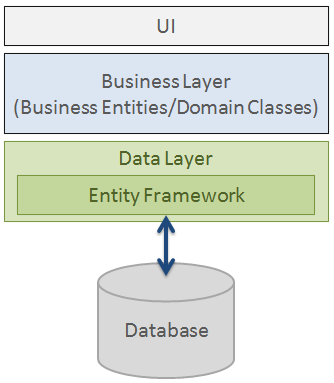
\includegraphics[width=6cm]{./IMAGENES/ef} 
		\caption{Entity Framework}
	\end{center}
\end{figure}

	\item \textbf{DataObjects.NET:} es un marco de mapeo de persistencia y relacional de objetos para Microsoft .NET. Permite a los desarrolladores definir objetos persistentes y lógica de negocios directamente en C\#, Visual Basic. Los objetos persistentes pueden ser recuperados por consultas LINQ. Los datos persistentes se pueden almacenar en servidores SQL. A diferencia de muchos otros marcos ORM, el modelo de base de datos se genera y mantiene automáticamente.\cite{do} \\
\end{itemize}



%% ----------------------------------------------------------------------------------------------------------------------------------
 


%% ANÁLISIS ( APLICACIÓN ) ---------------------------------------------------------------------------------------------------

\section{Análisis}

\subsection{\textbf{Herramientas ORM}}
Los ORM proporcionan una abstraccion de alto nivel
en una base de datos relacional que permite a un desarrollador escribir codigo Python en lugar de SQL para crear, leer, actualizar y eliminar datos y esquemas en su base de datos. Los desarrolladores pueden usar el lenguaje de programacion con el que se sienten comodos para trabajar con una base de datos en lugar de escribir sentencias de SQL o procedimientos almacenados.\\

\subsection{\textbf{Como ejemplo tenemos la herramienta Dapper}}
Dapper es un simple mapeador de objetos para .NET y posee el título de King of Micro ORM en términos de velocidad y es virtualmente tan rápido como usar un lector de datos en bruto ADO.NET. Un ORM es un Asignador Relacional de Objetos, que es responsable de la asignación entre la base de datos y el lenguaje de programación.
Dapper extiende la IDbConnection proporcionando métodos de extensión útiles para consultar su base de datos. \citep{DapperNet}

\subsection{\textbf{¿Como funciona?}}
\begin{itemize}
\item Crear un objeto IDbConnection.
\item Escribe una consulta para realizar operaciones de CRUD.
\item Pasar la consulta como un parámetro en el método de ejecución.
\end{itemize}

\subsection{\textbf{Metodos}}
\begin{itemize}
\item Ejecutar
\item Consulta
\item QueryFirst
\item QueryFirstOrDefault
\item QuerySingle
\item QuerySingleOrDefault
\item QueryMultiple
\end{itemize}

\begin{figure}
\begin{center}
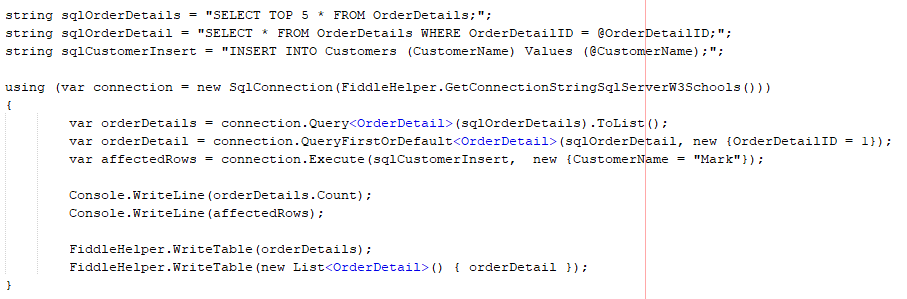
\includegraphics[width=14cm]{./Imagenes/Ejemplo}
\end{center}
\end{figure}

%% ----------------------------------------------------------------------------------------------------------------------------------


%% CONCLUSIONES ---------------------------------------------------------------------------------------------------------------

\section{Conclusiones}

\begin{itemize}

\item Conclusion 1 :  El mapeo objeto-relacional (ORM) es una técnica para mapear sistemas orientados a objetos a bases
de datos relacionales.Utilizar las diferentes herramientas de ORM, da mas rapidez y eficiencia a la construcción de base
de datos.\\

\item Conclusion 2 : ORM es imprescindible para poder trabajar con base de datos relacionales y
programación orientada a objetos, ya que es éste puede enlazar estas dos modalidades
de trabajo. Se podrán crear todas las consultas de base de datos que se desean. Gracias a esto nos ayuda a poder hacer consultas
sin la nesecidad de generar crear scripts en la base de datos, pero desde mi punto de vista los scripts son mas reusables que ORM.
Recomendaria usar el ORM para sistemas pqueños o para consultas especificas.
 
\item Conclusion 3 : \\ La utilización de mapeadores objeto/relacional brinda muchos beneficios para las aplicaciones que manejan un elevado volumen de datos y tienen una lógica de negocio compleja. Se debe tener en cuenta aspectos referentes a la performance de la aplicación durante las primeras etapas de diseño y en la definición de la arquitectura, dejando de lado los aspectos puros de diseño de objetos y relacional para rescatar lo positivo de cada uno y combinarlo para lograr mejores resultados.

\item Conclusion 4 : \\ 
\end{itemize}

%% ----------------------------------------------------------------------------------------------------------------------------------

%%  REFERENCIAS BIBLIOGRÁFICAS ------------------------------------------------------------------------------------------
	
	\newpage
	
	\bibliographystyle{apalike} 	%ESTILO
	\bibliography{BIBLIOGRAFIA}	 
	
	
\end{document}
